\phantom.
\vspace{3cm}
\section{Basic ground-state theory}\label{dft_sec}


\subsection{The many-body problem}
All physical properties of a solid-state material, consisting of $N$ electrons and $N_\text{K}$ nuclei, are fully described by a many-body wave function obeying a time-independent Schr\"odinger equation. However, solving the full equation is computational impossible as it depends on $3N + 3N_\text{K}$ spatial coordinates, that both are in the order of $10^{23}$.
Therefore, simplifications are needed in order to determine the wave function of the system. The first one usually made in this context is the Born-Oppenheimer approximation. It is based on the fact that the electron's mass is much smaller than the masses of the nuclei such that electronic and nuclear degrees of freedom can be separated. As a consequence, the electronic wave function can be determined  for a given nuclear configuration entering the equation only parametrically. After applying this approximation, it remains the following equation\footnote[2]{Throughout this thesis, atomic units are used, \textit{i.e.}, $\hbar=e=m_\text{e}=1$, where $\hbar$ is the reduced Planck constant, and $e$ and $m_e$ are the electron's charge and mass, respectively.}  describing the behavior of $N$ interacting electrons in the external field generated by the nuclei:
%
\begin{align}\label{born-op}
   \left[ -\sum_i\frac{\nabla^2_i}{2}  + \frac{1}{2}\sum_{i\neq j}\frac{1}{|\r_i - \r_j|} - \sum_{i,I}\frac{Z_I}{|\r_i - \R_I|}\right]\Psi(\r_1,\r_2,...,\r_N) = E\,\Psi(\r_1,\r_2,...,\r_N),
\end{align}
%
with the set of atomic numbers $\{Z_1,Z_2,...,Z_{N_\text{K}}\}$ and the sets of electronic coordinates  $\{\r_1,\r_2,...,\r_N\}$ nuclear coordinates $\{\R_1,\R_2,...,\R_{N_\text{K}}\}$. The summation indices in Eq.\;\eqref{born-op} are $i$ for the electrons and $I$ for the nuclei. The electronic wave function is denoted as $\Psi(\r_1,\r_2,...,\r_N)$. The first and second term describe the electrons' kinetic energy and their interaction among each other. They are universal operators for every system of~$N$ electrons, whereas the third term is an external potential $\hat{V}_\text{ext}$ that is caused by the nuclei and depends on the system to be studied. The external potential can be written as a sum of one-particle potentials $\hat{v}_\text{ext}$ according to
%
\begin{equation}
    \hat{V}_\text{ext} = \sum_i \hat{v}_\text{ext}(\r_i).
\end{equation}
%
Equation~\eqref{born-op} now depends on $3N$ spatial coordinates. A full solution, however, is still computationally not feasible due to the electron-electron interaction. An approach avoiding to find the full electronic wave function is density-functional theory, which shall be introduced in the following section.
%
\subsection{Density-functional theory}
Within the framework of density-functional theory (DFT), the  electronic ground-state (GS) density $ n_\text{GS}^{\phantom{I}}(\r)$, depending only on 3 variables, is used as a central object instead of the electronic wave function.  All observables can be defined as functionals of the density, which significantly reduces the computational effort as the solution of the full Schr\"odinger equation (Eq.\;\eqref{born-op}) can be avoided. \par
The legitimacy of DFT is given by the two theorems of Hohenberg and Kohn \cite{hk64}. The first Hohenberg-Kohn (HK) theorem states that there is a one-to-one correspondence between the external potential $\hat{v}_\text{ext}(\r)$ in Eq.\;\eqref{born-op} and the GS electronic density. As a result of this, the GS energy (in the following also referred to as the \textit{total energy}) of the system is also a functional of the GS density, which has the form
%
\begin{align}\label{e_func}
    E[n_\text{GS}^{\phantom{I}}] = \int\text{\!\!d}\r\, v_\text{ext}(\r)\,n_\text{GS}^{\phantom{I}}(\r)  + T[n_\text{GS}^{\phantom{I}}] + U[n_\text{GS}^{\phantom{I}}] = \int\text{\!\!d}\r\,v_\text{ext}(\r)\, n_\text{GS}^{\phantom{I}}(\r) + F[n_\text{GS}^{\phantom{I}}],
\end{align}
%
where $T[n]$ and $U[n]$ are universal functionals arising from the kinetic energy of the electrons and their interaction, respectively, and $F[n]$ is their sum. The second theorem states that the functional $E[n]$ is minimized if (and only if) the input density is the true GS density. To do actual computations, an explicit expression for $F[n]$ is needed, which is not yet given by the two theorems. One possible form was introduced by Kohn and Sham (KS)\cite{ks65} who proposed a separation of the functional into three parts:
%
\begin{align}\label{univ_func}
    F[n] = T_0[n] + E_\text{H}[n] + E_\text{xc}[n].
\end{align}
%
Thus, $F[n]$ is divided into the kinetic-energy functional of non-interacting electrons $T_0[n]$, the Hartree-energy $E_\text{H}[n]$ resulting from the  classical electrostatic interaction, and the exchange-correlation functional $E_\text{xc}[n]$ including all many-body quantum effects, which have not been accounted for. According to the second HK theorem, the functional derivative of $E[n]$ vanishes for the true GS density. Under the condition that the number of electrons $N$ is a constant, which can be ensured by introducing a Lagrange multiplier $\mu$, this leads to 
%
\begin{align}\label{minim}
    \delta E[n] = \int\text{\!\!d}\r\left[ \frac{\delta T_0[n]}{\delta n(\r)} + v_\text{KS}^{\phantom{I}}(\r) - \mu \right] \delta n(\r) = 0.
\end{align}
%
In this equation, the effective KS potential $v_\text{KS}^{\phantom{I}}(\r)$ is given by 
%
\begin{align}
   v_\text{KS}^{\phantom{I}}(\r) =  v_\text{ext}(\r)+\int\text{\!\!d}\r'\frac{n(\r')}{|\mathbf{r-r'}|} + \frac{\delta E_\text{xc}[n]}{\delta n(\r)}.
\end{align}
%
Equation~\eqref{minim} also holds for a system of non-interacting electrons in an effective external potential $v_\text{KS}^{\phantom{I}}(\r)$. Consequently, the problem of finding the GS density of a system of $N$ interacting electrons in an external potential can be reformulated as finding the GS density of a system of $N$ non-interacting electrons in the effective KS potential.
The GS density can therefore be obtained  by solving $N$ single-particle Schr\"odinger equations, also referred to as the KS equations:
%
\begin{align}\label{kseq}
\left[ -\frac{\nabla^2}{2} + v_\text{KS}^{\phantom{I}}(\r) \right] \psi_i(\r) = \varepsilon_i\,\psi_i(\r).
\end{align}
%
The set of single-particle wave functions $\{\psi_1,\psi_2,...\psi_N\}$ yields the GS density of the interacting system as
%
\begin{align}
    n_\text{GS}^{\phantom{I}}(\r) = \sum^N_{i=1}|\psi_i(\r)|^2.
\end{align}
%
Since the density itself also depends on the single-particle wave functions, Eq.\;\eqref{kseq} has to be solved self-consistently until sufficient convergence is reached. From their definition, it is clear that there is no physical meaning associated with the KS eigenvalues. However, they are often interpreted as electronic single-particle energies\cite{gw_method} defining the KS band structure.\par
%
When solving Eq.\;\eqref{kseq} for periodic crystals, one can take advantage of the invariance of $v_\text{KS}^{\phantom{I}}(\r)$ under a translation by any lattice vector  $\r$, \textit{i.e.}, $v_\text{KS}^{\phantom{I}}(\r)=v_\text{KS}^{\phantom{I}}(\mathbf{r+R})$. In this case, according to Bloch's theorem, the electronic wave function of a band $i$ at a wavevector $\k$ takes the form $\psi_{i\k}(\r)=e^{i\mathbf{k\cdot r}}u_{i\k}(\r)$, where $u_\k(\r)$ is a lattice-periodic function. In infinite systems, $\k$ is a continuous quantity. For practical calculations, however, the system is assumed to be finite, consisting of $N_p$ copies of the unit cell, which also restricts the wavevector to a finite number of $N_p$ $\k$-points. Besides the band index, the wavevector therefore becomes a second quantum number.\par
\newpage
So far, all unknown information about the many-body system was put into the exchange-correlation functional for which plenty of approximations have been developed over the last decades. The most prominent classes are the local-density (LDA) and the generalized gradient approximations (GGA)\cite{bechstedt2016many}. In LDA, the exchange-correlation functional depends only on the density $n(\r)$ and can be expressed as 
%
\begin{align}
    E^\text{LDA}_\text{xc}[n] = \int\text{\!\!d}\r\,e_\text{xc}\bigl(n(\r)\bigr)\,n(\r),
\end{align}
%
where $e_\text{xc}$ is the exchange-correlation energy per particle of the homogeneous electron gas at constant density. In GGA, the functional depends additionally on the  gradient of the density $|\nabla n(\r)|$. Despite the success of LDA or GGA for many systems, it has been shown that the standard methods for the calculation of electronic spectra based on those approximations break down in materials with strong electron correlation\cite{rpa_correlation_energies}. Therefore, higher level functionals have been developed, that are dependent on occupied or on both occupied and unoccupied orbitals. Using orbital-dependent functionals, the exchange interaction in molecules can be treated exactly\cite{exact_exchange,exact_exchange2}, while  accurate expressions for the correlation functional can be obtained from many-body perturbation theory\cite{mbpt_correlation,mbpt_correlation2}.\par


\subsection{The LAPW+lo method}

To numerically solve Eq.\;\eqref{kseq}, the KS wave functions are expanded in a basis. Among many possibilities of choosing a basis, the use of linearized augmented plane waves and local orbitals (LAPW+lo) is widely considered to be the \textit{gold standard} of DFT for extended systems, as they allow for solving the KS equations  with high precision\cite{exciting}.  The expansion of the KS wave functions in basis functions $\phi_\mathbf{G+k}$ and coefficients $C^\G_{i\k}$  reads
 %
 \begin{align}
    \psi_{i\k}(\r) = \sum_\G C^\G_{i\k}\,\phi_\mathbf{G+k}(\r),
\end{align}
%
where the sum runs over reciprocal lattice vectors $\G$.  Within the LAPW framework, the unit cell is divided into two distinct regions, one being the muffin-tin spheres (MT): These are spheres centered at each atomic position $\r_\alpha$, having a radius $R_{\text{MT},\alpha}$ such that spheres around different atoms do not overlap.  The basis functions are given by
 %
 \begin{align}\label{basis}
     \phi_\mathbf{G+k}(\r) = \begin{cases}
      \sum\limits_{lm}A^{\mathbf{G+k}}_{lm\alpha}\,u_{l\alpha}(r_\alpha)\,Y_{lm}(\hat{\r}_\alpha), & \text{if } r_\alpha \leq R_{\text{MT},\alpha} \\
      \frac{1}{\sqrt{V}}\,e^{i(\mathbf{G+k})\cdot\r}, & \text{if }  \r \in I.
    \end{cases}
 \end{align}
 %
 Inside the muffin-tin spheres, an expansion into spherical harmonics  $Y_{lm}(\hat{\r}_\alpha)$ and radial functions  $u_{l\alpha}(r_\alpha)$ as functions of the variable $\r_\alpha = \mathbf{r-R_\alpha}$ is employed.  The remaining part of the unit cell is called the interstitial region $I$ where plane-waves are used.
The coefficients  $A^{\mathbf{G+k}}_{lm\alpha}$ are determined imposing continuity of the basis functions at the sphere boundary. A major advantage of this procedure is its capability of accurately describing the wave functions in the vicinity of the nuclei (where they are strongly varying) and their smooth and slowly varying behavior elsewhere.\par
Assuming that the KS potential  $v_\text{KS}^{\phantom{I}}(\r)$ is spherically symmetric inside the muffin-tin sphere, it can be replaced by its spherical average $v_0(r)$. With this assumption, the radial functions $u_{l\alpha}(r)$ are required to obey the radial Schr\"odinger equation
 %
 \begin{align}\label{radfunc}
     \left[ -\frac{1}{2}\frac{\text{d}^2}{\text{d}r^2} + \frac{l(l+1)}{2r^2} + v_0(r) - \varepsilon_{i\k}\right]\bigl(r\,u_{l\alpha}(r)\bigr) = 0.
 \end{align}
 %
  From here, it follows that the basis functions defined in Eq.\;\eqref{basis} themselves depend on the energy-eigenvalues $\varepsilon_{i\k}$ resulting in a non-linear eigenvalue-problem. To overcome this difficulty, Eq.\;\eqref{radfunc} is linearized by choosing  fixed energies $\varepsilon_{l\alpha}$. The resulting error can be reduced  in the spirit of an expansion in the energies by approximating  the radial functions as
  %
  \begin{align}
    u_{l\alpha}(r_\alpha,\varepsilon) = u_{l\alpha}(r_\alpha,\varepsilon_{l\alpha}) + \Dot{u}_{l\alpha}(r_\alpha,\varepsilon_{l\alpha})\,[\varepsilon_{l\alpha} - \varepsilon],
  \end{align}
  where $\Dot{u}_{l\alpha}(r_\alpha,\varepsilon_{l\alpha})=\partial u_{l\alpha}(r_\alpha,\varepsilon) /\partial\varepsilon$.
%
This leads to  the linearized augmented plane-wave (LAPW) basis where the part of the basis corresponding to the MT part changes from the definition in Eq.\;\eqref{basis} to 
  %
  \begin{align}
      \phi_\mathbf{G+k}(\r) =  \sum\limits_{lm}\left[A^{\mathbf{G+k}}_{lm\alpha}\,u_{l\alpha}(r_\alpha;\varepsilon_{l\alpha}) + B^{\mathbf{G+k}}_{lm\alpha}\,\dot{u}_{l\alpha}(r_\alpha;\varepsilon_{l\alpha}) \right]\,Y_{lm}(\hat{\r}_\alpha). 
  \end{align}
 %
 Again, the expansion coefficients $A^{\mathbf{G+k}}_{lm\alpha}$ and $B^{\mathbf{G+k}}_{lm\alpha}$ are obtained requiring the continuity of the basis and its spatial derivative at the boundaries of the MT spheres.  A different method proposed to linearize the problem is the additional use of local orbitals\cite{apw+lo}. These are basis functions being only non-zero inside the MT sphere and defined by 
 %
 \begin{align}
    \phi_\mu(\r) = \begin{cases}
      \delta_{\alpha\alpha_\mu}\delta_{ll_\mu}\delta_{mm_\mu}[a_\mu \,u_{l\alpha}(r_\alpha;\varepsilon_{l\alpha}) +b_\mu\, \dot{u}_{l\alpha}(r_\alpha;\varepsilon_{l\alpha})]\,Y_{lm}(\hat{\r}_\alpha), & \text{if } r_\alpha \leq R_{\text{MT},\alpha} \\
      0, & \text{if }  \r \in I.
      \end{cases}
  \end{align}
 %
  The coefficients $a_\mu, b_\mu$ are chosen such that the local orbital is normalized and vanishes at the MT boundary. The use of local orbitals gives a highly-flexible basis set, which can be adjusted to each specific system. 

 %-------------
\subsection{Phonons in polar materials}\label{pol_phon}
%-------------
The central quantities in the calculation of phonons are the matrix of the interatomic force constants (IFCs) and the dynamical matrix. The matrix of the IFCs is defined as  the second derivative of the total energy  $E$ with respect to the atomic displacements:
%
\begin{align}
  C_{\kappa\alpha p}^{\kappa'\alpha'p'} = \left.\frac{\partial^2E}{\partial\tau_{\kappa\alpha p}\,\partial\tau_{\kappa'\alpha'p'}}\right\vert_0,
\end{align}
%
where $\vert_0$ means that the derivative is taken at the equilibrium configuration with vanishing forces and stresses. The displacement of the atom $\kappa$ from its equilibrium position in direction $\alpha$ in the cell $p$ with vector $\r_p$ is denoted by $\tau_{\kappa\alpha p}$. The Fourier transform of $C$ is defined as 
%
\begin{align}
    \tilde{C}_{\kappa\alpha}^{\kappa'\alpha'\!}(\q) =\sum_p C_{\kappa\alpha0}^{\kappa'\alpha' p}\,\exp(i\,\q\cdot\r_p),
\end{align}
%
 and is related to the dynamical matrix by $\tilde{D}_{\kappa\alpha}^{\kappa'\alpha'\!}(\q) = \tilde{C}_{\kappa\alpha}^{\kappa'\alpha'\!}(\q)/\sqrt{M_\kappa M_{\kappa'}}$, where $M_\kappa$ is the mass of the $\kappa$th nucleus. The squares of the phonon frequencies $\omega_{\nu}(\q)$ of a mode $\nu$ and the corresponding eigendisplacements $e_{\kappa\alpha\nu}(\q)$ are obtained by diagonalizing the dynamical matrix according to
 %
 \begin{align}
     \sum_{\kappa'\alpha'} \tilde{D}_{\kappa\alpha}^{\kappa'\alpha'\!}(\q)\,e_{\kappa'\alpha'\nu}(\q) =  \omega^2_{\nu}(\q)\,e_{\kappa\alpha\nu}(\q).
 \end{align}
%
At the Brillouin-zone (BZ) center, as well as along high-symmetry directions in the BZ, the phonon modes can be separated into longitudinal and transverse modes. Additionally, they can be classified into optical and acoustical phonons by the movement of the atoms relative to each other. Optical modes correspond out-of-phase movements of the atoms in the lattice  where neighbouring atoms move in opposite directions whereas acoustical modes displace the atoms in the same direction. For a material with $N_\text{at}$ atoms in the unit cell, there exist $3N_\text{at}$ modes in total, 3 acoustical of which two are transverse (TA) and one is longitudinal (LA). The remaining $3N_\text{at}-3$ modes are transverse (TO) and longitudinal (LO) optical modes.\footnote[2]{Although a strict separation in LA and TA as well as LO and TO modes is only possible at $\Gamma$ and along high-symmetry directions, these labels are extended to the corresponding modes over the whole~BZ.}\par
In polar materials, the atoms carry non-zero Born effective charge tensors $\mathbf{Z}^*_\kappa$, which are defined as the derivative of the polarization $\mathbf{P}$ per unit cell   with respect to the atomic displacements:
%
\begin{equation}
    Z^*_{\kappa,\alpha\beta} = \Omega_\text{UC}\,\left.\frac{\partial P_\beta}{\partial\tau_{\kappa\alpha}}\right\vert_0.
\end{equation}
%
\newpage
In this equation, $\Omega_\text{UC}$ is the unit-cell volume and the derivative has to be evaluated at zero displacement, which is denoted by $\vert_0$. Due to the Born effective charges, longitudinal optical modes are accompanied by macroscopic electric fields in the long wavelength limit $\q\rightarrow0$. These electric fields result in an additional restoring Coulomb force, which is not present for transverse optical modes. Therefore, the LO frequencies $\omega^{\phantom{I}}_\text{LO}$ increase at the Brillouin zone center above those of the corresponding TO frequency $\omega^{\phantom{I}}_\text{TO}$, which is known as LO-TO splitting\cite{cardona2005fundamentals}. A convenient way of dealing with this problem in the computation of long-wavelength phonons is to exploit the known analytic properties of the dynamical matrix\cite{pavone_phonons}. In the long-wavelength limit, the force-constants $\tilde{C}$ can be separated into two contributions, one being analytical (an), the other nonanalytical~(na):
%
\begin{align}
    \tilde{C}_{\kappa\alpha}^{\kappa'\alpha'}(\q\rightarrow0) = \left[\tilde{C}_{\kappa\alpha}^{\kappa'\alpha'}(\q=0)\right]^\text{an} + \left[\tilde{C}_{\kappa\alpha}^{\kappa'\alpha'}(\q\to 0)\right]^\text{na}.
\end{align}
%
The analytical part is obtained from the response to a long-wavelength phonon, calculated under the use of boundary conditions corresponding to zero macroscopic electric field. The nonanalytical part is given by\cite{pavone_phonons}
%
\begin{align}\label{forceconst_an}
   \left[\tilde{C}_{\kappa\alpha}^{\kappa'\alpha'}(\q\to 0)\right]^\text{na\!\!} = \frac{4\pi}{\Omega_\text{UC}}\frac{(\q\cdot \mathbf{Z}^*_\kappa)_\alpha\,(\q\cdot \mathbf{Z}^*_{\kappa'})_{\alpha'}}{\mathbf{q\cdot\boldsymbol{\varepsilon}_\infty \cdot q}}.
\end{align}
%
 If the eigendisplacements of $\tilde{C}(\q\rightarrow0)$ are identical to those of $\tilde{C}(\q=0)$, which is the case for instance in cubic crystals, the LO and TO frequencies of a mode $\nu$ are linked by\cite{gonze_lee}
%
\begin{align}\label{w_loto_split}
    \omega^2_\nu(\q\rightarrow0) =\overline{\omega}^2_{\nu 0} + \frac{4\pi}{\Omega_\text{UC}}\,\frac{|\hat{\q}\cdot\mathbf{Q}_{\nu}|^2}{\q\cdot\boldsymbol{\varepsilon}_\infty\cdot\q},
\end{align}
%
where $\boldsymbol{\varepsilon}_\infty$ is the pure electronic static dielectric tensor  (further discussed in Section~\ref{subsec_lin_response}), and $\overline{\omega}_{\nu 0} = \left[\omega_\nu(\q=0)\right]^\text{an}$ denotes the phonon frequency corresponding to the analytical part of the force constants at $\q=0$. The polarization vector $\mathbf{Q}_{\nu}$ is defined as
%
\begin{align}\label{pol_vec}
    \mathbf{Q}_{\nu}(\q) & = \sum_{\kappa} \frac{1}{\sqrt{M_\kappa }}\,\mathbf{Z}^*_\kappa\cdot \mathbf{e}_{\kappa\nu}(\q).
\end{align}
%
The macroscopic electric fields associated with long wavelength LO phonons do not only modify the phonon frequencies, but also result in a contribution of the ions to the dielectric tensor. The full static dielectric tensor, $\boldsymbol{\varepsilon}_0$, is obtained by adding the ionic contribution to  $\boldsymbol{\varepsilon}_\infty$ according to\cite{gonze_lee}
%
\begin{align}\label{eps_w_relation}
    \varepsilon_{0,\alpha\beta} = \varepsilon_{\infty,\alpha\beta} + \frac{4\pi}{\Omega_\text{UC}}\sum_\nu\frac{Q_{\nu,\alpha}Q_{\nu,\beta}}{\overline{\omega}^2_{\nu 0}}.
\end{align}
%
In cubic materials, the dielectric tensors are diagonal and have only one independent element each, which are denoted as $\varepsilon_\infty$ and $\varepsilon_0$. In the case of a diatomic basis, where \newpage only one LO mode exists, LO and TO frequencies ($\omega^{\phantom{I}}_\text{LO}$ and $\omega^{\phantom{I}}_\text{TO}$) are connected with the dielectric constants by the famous Lyddane-Sachs-Teller relation\cite{lst_rel}. It states that
%
\begin{align}\label{lst}
    \frac{\varepsilon_0}{\varepsilon_\infty} = \left(\frac{\omega^{\phantom{I}}_\text{LO}}{\omega^{\phantom{I}}_\text{TO}}\right)^{\!\!2}.
\end{align}
 %
From Eqs.~\eqref{w_loto_split} and \eqref{eps_w_relation}, it becomes clear that both  LO-TO splitting and the ionic contribution to the dielectric tensor will not be present in non-polar materials where all Born-effective charges vanish.
 \newpage
 %-----------------------
 %-----------------------
 \phantom.
\vspace{3cm}
 \section{Many-body perturbation theory}\label{mbpt_sec}
 %-----------------------
 %-----------------------

 In the previous chapter, the ideas behind density-functional theory (DFT) for calculating ground-state properties and phonons were discussed. While electron-phonon interactions (EPI) can be treated within density-functional perturbation theory\cite{dfpt1,dfpt2}, the computation of excited states, being responsible for the optical properties of a system\cite{bechstedt2016many}, is notoriously difficult within the traditional DFT approach of Kohn and Sham\cite{Gross1996}. Consequently, a more general framework is required in order to account for the effects of EPI on excited states.\par A rigorous mathematical treatment aiming at the description of both excited states and electron-phonon interactions from first principles is many-body perturbation theory (MBPT), which will be briefly reviewed in this section. A central idea of MBPT is the introduction of \textit{quasiparticles}, effective single-particle states, which are ``dressed'' by the interaction with the many-body system. Excitations can then be described in terms of interacting quasiparticles, which simplifies the computation compared to the evaluation of the whole many-body system. The concept of quasiparticles is embedded in a description through Green's functions, which accordingly are central quantities of the theory\cite{fetterwalecka}. The single-particle Green's function, for instance, reveals information about the single-particle excitation spectrum.\par
For the calculation of optical properties, also the knowledge of two-particle excitations is required since interactions between quasielectrons and quasiholes come into play. These excitations are contained in the two-particle Green's function and a related quantity, the correlation function. A widely used method to account for two-particle excitations is the solution of the  Bethe-Salpeter equation (BSE), which is the equation of motion of the correlation function\cite{sagmeister}. The BSE can be reformulated as an eigenvalue problem by introducing an effective two-particle Hamiltonian with an interaction part consisting of a screened Coulomb term (also referred to as direct term) and an exchange term. The eigenvalues and eigenfunctions of this Hamiltonian are closely related to the optical spectrum.
\subsection{Electron-phonon interactions (EPI)}\label{subsec_epc}
%----------------------------

\subsubsection{The electron-phonon coupling Hamiltonian}
The Hamiltonian describing the coupled system of electrons and phonons is given by\cite{Giustino}
%
\begin{equation}\label{eph_ham}
  \begin{aligned}
    \hat{H}  = & \sum_{n\k} \varepsilon_{n\k}\,\hat{c}^\dagger_{n\k}\,\hat{c}_{n\k} + \sum_{\q\nu}\hbar\omega_{\q\nu}\,\left(\hat{a}^\dagger_{\q\nu}\,\hat{a}_{\q\nu} + \tfrac{1}{2}\right) \\[10pt]
    & + \frac{1}{\sqrt{N_p}}\sum_{\substack{\k,\q \\ mn\nu}}g_{mn\nu}(\k,\q)\,\hat{c}^\dagger_{m\mathbf{k+q}}\,\hat{c}_{n\k}\,\left(\hat{a}_{\q\nu} + \hat{a}^\dagger_{-\q\nu}\right).\\[10pt]
    %& + N_p^{-1}\sum_{\substack{\mathbf{k,q,q'} \\ mn\nu\nu'}}g^\text{DW}_{mn\nu\nu'}(\mathbf{k,q,q'})\hat{c}^\dagger_{m\mathbf{k+q}}\hat{c}_{n\k}(\hat{a}_{\q\nu} + \hat{a}^\dagger_{\mathbf{-q}\nu})(\hat{a}_{\mathbf{q'}\nu'} + \hat{a}^\dagger_{\mathbf{-q'}\nu'}).
\end{aligned}  
\end{equation}
%
In this equation, the first line stems from the separate electron and phonon subsystems. $\varepsilon_{n\k}$ is the single-particle eigenvalue of an electron in the band $n$, carrying crystal momentum $\k$. The eigenvalues are obtained by solving the Kohn-Sham equations as given in Eq.\;\eqref{kseq}. Compared to preceding section, the notation $\omega_{\q\nu}\equiv\omega_{\nu}(\q)$ was introduced for the frequency of a lattice vibration in the mode $\nu$ carrying crystal momentum $\q$. The pairs ($\hat{c}^\dagger_{n\k},\hat{c}_{n\k}$) and ($\hat{a}^\dagger_{\q\nu},\hat{a}_{\q\nu}$) are creation and annihilation operators associated to fermionic and bosonic fields, respectively. $N_p$ is the number of unit cells in the crystal. The second line in Eq.\;\eqref{eph_ham} accounts for the coupling between electrons and phonons to first order in the atomic
displacements. The electron-phonon interaction (EPI) is expressed in terms of the EPI matrix element $g_{mn\nu}(\k,\q)$, which specifies the coupling strength.

\subsubsection{The electron-phonon matrix element}
The matrix element of EPI depends on the crystal momenta of the participating particles and has the physical dimension of an energy. Formally, it is defined by 
%
\begin{align}\label{g_formal}
    g_{mn\nu}(\mathbf{k,q}) &  =\mel{\psi_{m\mathbf{k+q}}}{\Delta^{\!\q\nu}v_\text{KS}^{\phantom{I}}}{\psi_{n\k}}.
\end{align}
%
This expression can be seen as the probability amplitude for the scattering of an electron in  $\psi_{n\k}$ into the state $\psi_{m\mathbf{k+q}}$ due to a perturbation of the KS potential $\Delta^{\!\q\nu}v_\text{KS}^{\phantom{I}}$ caused by a phonon in the mode $\nu$ carrying crystal momentum $\q$. This process is depicted in Figure~\ref{mel_elph}.\par
\newpage
In order to account for the electron-phonon coupling in real space, one can define the
 screened electron-phonon coupling functions $g_{\q\nu}(\r,\omega)$ and $g^\text{cc}_{\q\nu}(\r,\omega)$ by
%
\begin{align}
         g_{\q\nu}(\r,\omega) & = \int_V\text{\!\!d}\r' \,\varepsilon_\text{el}^{-1}(\r,\r',\omega)\,\Delta^{\!\q\nu}v_\text{ext}^{\phantom{I}}(\r),\label{eph_coupl_func}\\[10pt]
         g^\text{cc}_{\q\nu}(\r,\omega) & = \int_V\text{\!\!d}\r' \,\varepsilon_\text{el}^{-1}(\r,\r',\omega)\left[\Delta^{\!\q\nu}v_\text{ext}^{\phantom{I}}(\r)\right]^*\label{eph_coupl_func_cc}, 
\end{align}
%
where $\varepsilon_\text{el}^{-1}$ is the electronic contribution to the inverse dielectric function (see Section~\ref{subsec_lin_response}), and $\Delta^{\!\q\nu}v_\text{ext}^{\phantom{I}}$ the perturbation of the external potential. With the definition in Eq.\;\eqref{eph_coupl_func}, the electron-phonon matrix element can be rewritten as\cite{Giustino}
%
%
\begin{align}\label{g_coupl_func}
    g_{mn\nu}(\mathbf{k,q}) &  =\mel{\psi_{m\mathbf{k+q}}}{ g_{\q\nu}(\r,\omega)}{\psi_{n\k}}.
\end{align}
%
A common approximation is to  neglect the frequency dependence of the screened coupling function by setting $g_{\q\nu}(\r,\omega)\approx g_{\q\nu}(\r,0)$.
\begin{figure}[t]
\centering
\begin{tikzpicture}
\begin{feynman}
\vertex (a) {$m\k+\q$};
\vertex [left=4cm of a] (b)  { \large{$g_{mn\nu}(\mathbf{k,q})$} $\longrightarrow$};
\node[left=2cm of a,draw,fill=black,dot] (b);
\vertex [above left= 2cm of b] (f1) {$n\mathbf{k}$};
\vertex [below left=2cm of b] (c) {$\q\nu$};

\diagram* {
(f1) -- [fermion] (b) -- [fermion] (a),
(b) -- [boson] (c),

};
\end{feynman}
\end{tikzpicture}
\caption{Diagrammatic representation of the electron-phonon scattering process.}
\label{mel_elph}
\end{figure}
%------------------------------------
\subsubsection{Fr\"ohlich coupling}\label{subsec_frohlich}
%------------------------------------

In general, the EPI matrix element has to be obtained numerically by evaluating Eq.\;\eqref{g_formal}. However,  for polar materials, where two or more atoms in the unit cell carry non-zero Born effective charge tensors, an analytic expression can be derived. Due to the Born charges,  atomic displacements associated with longitudinal optical (LO) phonon modes generate macroscopic electric fields. These fields, in turn, can strongly couple to charge carriers like electrons and holes. An early model of describing this type of electron-phonon coupling was given by Fr\"ohlich\cite{froehlich} who assumed an electron in a parabolic band interacting with one dispersionless LO phonon in an isotropic material. The resulting matrix element is given by 
 %
        \begin{equation}
        g^\text{F\!}(\q) = \frac{i}{|\q|}\left[\frac{4\pi}{\Omega_\text{UC}}\frac{\omega^{\phantom{I}}_\text{LO}}{2}\left(\frac{1}{\varepsilon_\infty} - \frac{1}{\varepsilon_0}\right)\right]^\frac{1}{2},
        \end{equation}
%       
where $\varepsilon_\infty$ and $\varepsilon_0$ are the macroscopic dielectric constants (see Eq.\;\eqref{epsmac} for a formal definition) and $\omega^{\phantom{I}}_\text{LO}$  is the LO phonon frequency. The interaction between electrons and phonons diverges for large wavelengths ($\q\rightarrow0$) and vanishes for large $\q$. Compared to the general definition of the electron-phonon matrix element in Eq.\;\eqref{g_formal}, it should be noted that the Fr\"ohlich coupling is not depending on the electron wave vector $\k$ and on the band indices (since only one electronic band is considered).
\subsection{The electron self-energy}

%
 %------------------
 \subsubsection{The single-particle Green's function}\label{green_subsec}
 %---------------------------------------------------------------------
 %
 Introducing combined indices of the form $ 1\equiv(\mathbf{x}_1,t_1)$, the single-particle Green's function $G$ at zero temperature is defined as the expectation value 
 %
 \begin{align}\label{green}
     G(1,2) = -i\mel{0}{\hat{T}\,\hat{\psi}(1)\,\hat{\psi}^\dagger(2)}{0},
 \end{align}
 %
 where $\hat{T}$ is Wick's time-ordering operator and $\hat{\psi}$ is a fermionic field operator. Green's functions are also called propagators, as they express correlations between particles created (annihilated) at a given point in space and time and annihilated (created) at a different point. Depending whether $t_1>t_2$ or $t_2>t_1$, the single-particle Green's function describes the probability amplitude of the propagation of an electron or a hole, respectively.\par 
 The fully interacting Green's function $G$ can be linked to the Green's function of non-interacting particles $G_0$ through the Dyson equation
%
 \begin{align}\label{dyson}
     G(1,2) = G_0(1,2) + \int\text{\!\!d}(34)\,G_0(1,3)\,\Sigma(3,4)\,G(4,2),
 \end{align}
 %
which can be represented in terms of Feynman diagrams as shown in Figure~\ref{dyson_eq}. In this equation, $\Sigma$ is the self-energy, a non-local and energy-dependent function describing all exchange and correlation effects due to the interaction of an electron with the many-body system\cite{reining_int_el}. Within the scope of this thesis, in particular the couplings to electrons and phonons are relevant.  The self-energy therefore takes the form
%
\begin{align}\label{self_split}
    \Sigma(1,2) = \Sigma^\text{el}(1,2) + \Sigma^\text{ph}(1,2),
\end{align}
%
where $\Sigma^\text{el}$ and $\Sigma^\text{ph}$ are the self-energy contributions arising from electron-electron and electron-phonon interactions, respectively. When considering only   $\Sigma^\text{el}$, the effects of the vibrating lattice on the electron are completely neglected, which is known as clamped-nuclei approximation. For a non-interacting system, the self-energy vanishes, and the interacting and non-interacting Green's functions are equivalent. 
\begin{figure}[t]
\centering
  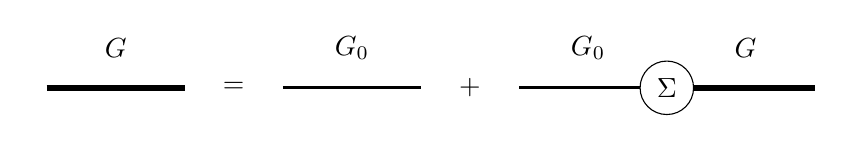
\begin{tikzpicture}[node distance=2cm,middlearrow/.style 2 args={
        decoration={             
            markings, 
            mark=at position 0.5 with {\arrow{triangle 45}, \node[#1] {#2};}
        },
        postaction={decorate}
    },
]
    %labels
    \node (g) {$G$};
    \node (equal) [right of=g,xshift=-.5cm,yshift=-0.5cm] {=};
    \node (g0) [right of=g,xshift=1cm] {$G_0$};
    \node (plus) [right of=g0,xshift=-.5cm,yshift=-0.5cm] {+};
    \node (g02) [right of=g0,xshift=1cm] {$G_0$};
    \node (g2) [right of=g02] {$G$};
    %cvertices
    \node (fullstart) [below of=g,xshift=-1cm,yshift=1.5cm]{};
    \node (fullend) [right of=fullstart]{};
    \node (nonstart) [below of=g0,xshift=-1cm,yshift=1.5cm]{};
    \node (nonend) [right of=nonstart]{};
     \node (nonstart2) [below of=g02,xshift=-1cm,yshift=1.5cm]{};
    \node (sigma) [right of=nonstart2,draw,fill=white,circle,]{$\Sigma$};
    \node (fullend2) [right of=sigma]{};
    
    %Pfeile
    \draw [line width = 2pt]  (fullstart) -- node {\fullarrow} (fullend);
    \draw [line width = 1pt] (nonstart) -- node {\nonintarrow} (nonend);
    \draw [line width = 1pt] (nonstart2) -- node {\nonintarrow} (sigma);
    \draw [line width = 2pt] (sigma) -- node {\fullarrow} (fullend2);
  \end{tikzpicture}
 \caption[Diagrammatic representation of the Dyson equation.]{Diagrammatic representation of the Dyson equation. The thick line represents the fully interacting Green's function $G$, the thin line corresponds to the non-interacting $G_0$.\label{dyson_eq}}
\end{figure}
 
%--------------------------------------
\subsubsection{Band structure renormalization}\label{subsec_renorm}
%--------------------------------------

The electronic eigenenergies computed including many-body effects through the evaluation of the self-energy constitute the quasiparticle band structure. The quasiparticle eigenvalues $\varepsilon^\text{QP}_{n\k}$ differ from the eigenvalues $\varepsilon_{n\k}$, which are obtained within the KS-DFT framework. It can  be shown\cite{hybertsen1986electron} that in a single-shot $G_0W_0$ approximation the eigenvalues of the two approaches are connected by
%
\begin{equation}
    \varepsilon^\text{QP}_{n\k} = \varepsilon_{n\k} + Z_{n\k}\left[\Re \Sigma_{n\k}(\varepsilon_{n\k}) - v^\text{xc}_{n\k}  \right],
\end{equation}
%
where the operators of the self-energy and the exchange-correlation potential are evaluated in the basis of the KS states according to
%
\begin{align}
   \Sigma_{n\k}(\varepsilon_{n\k}) & =\mel{n\k}{\hat{\Sigma}(\varepsilon_{n\k})}{n\k}\\[10pt]
   v^\text{xc}_{n\k} & = \mel{n\k}{\hat{v}_\text{xc}}{n\k}.
\end{align}
%
The renormalization factor $Z_{n\k}$ accounts for the energy-dependence of the self-energy. A simple approximation of the many-body correction to the KS band-structure is the use of a scissor operator, which rigidly shifts the KS eigenvalues. The quasiparticle band-structure within this approach is accordingly obtained by
\begin{equation}
    \varepsilon^\text{QP}_{n\k} = \varepsilon_{n\k} + \Delta,
\end{equation}
% 
where the scissor parameter $\Delta$ is chosen such that the fundamental quasiparticle band gap equals the experimental one.
%
\vfill%----------------
\subsubsection{Electronic contribution}\label{selfen_el}
%----------------

\begin{figure}[t]
\centering
\begin{tikzpicture}
\begin{feynman}
\node (a);
\vertex[blob,fill=white,right=3cm of a,very thick] (b){$\Gamma$};
\vertex [above=1.9cm of a, xshift = 1.5cm] {$W^\text{el}$};

\diagram* {
(a.center) -- [scalar,very thick, half left] (b) , (a.center) -- [fermion, very thick,edge label'=$G$] (b)

};
\end{feynman}
\end{tikzpicture}
\caption[Feynman diagram of the electronic contribution to the electron self-energy.]{Feynman diagram of the electronic contribution to the electron self-energy expressed in terms of the fully
interacting electron Green’s function $G$ (straight line), the
electronic screened Coulomb interaction $W^\text{el}$ (dashed line), and the vertex $\Gamma$ from~Eq.\;\eqref{vertex}.\label{el_self_en}}
\end{figure}
%
The electronic contribution to the self-energy can be obtained in principle by self-consistently solving the closed set of Hedin's equations\cite{hedin1965new}:
%
 \begin{align}
      \Sigma^\text{el}(1,2) & = i\int\text{\!\!d}(34)\,G(1,4)\,W^\text{el}(3,1^+)\,\Gamma(4,2,3)\label{sigma_el}\\
    W^\text{el}(1,2) & = v_\text{C}^{\phantom{I}}(1,2) + \int\text{\!\!d}(34)\,v_\text{C}^{\phantom{I}}(1,3)\, P^{\hspace{.2mm}\text{el}}(3,4)\,W^\text{el}(4,2) \label{dyson_w}\\
     \Gamma(1,2,3) & = \delta(1,2)\,\delta(1,3) + \int\text{\!\!d}(4567)\,\frac{\delta\Sigma(1,2)}{\delta G(4,5)}\,G(4,6)\,G(7,5)\,\Gamma(6,7,3)\label{vertex}\\
     P^{\hspace{.2mm}\text{el}}(1,2) & = -i\int\text{\!\!d}(34)\,G(1,3)\,G(4,1^+)\,\Gamma(3,4,2).
 \end{align}
 %
In these equations, $ P^{\hspace{.2mm}\text{el}}$ is the electronic polarizability, $W^\text{el}$ the screened Coulomb interaction due to electrons, and $\Gamma$ is the vertex function. The bare Coulomb interaction is denoted as  $v_\text{C}^{\phantom{I}}$. The notation \ldq$1^+$\rdq~indicates that the corresponding time~$t_1$ is infinitesimally later than the one of the combined index without the superscript. The electronic contribution to the self-energy can be depicted by the Feynman diagram shown in Fig.~\ref{el_self_en}.

Equation\;\eqref{dyson_w} for the screened Coulomb interaction can be rewritten by introducing the electronic part of the inverse dielectric function $ \varepsilon_\text{el}^{-1}$ (see also  Eq.\;\eqref{diel_pol}) by
 %
 \begin{equation}\label{epsel_pol}
         \varepsilon_\text{el}^{-1}(1,2) = \delta(1,2) - \int\text{\!\!d}(3)\,v_\text{C}^{\phantom{I}}(1,3)\, P^{\hspace{.2mm}\text{el}}(3,2).
 \end{equation}
 The screened Coulomb interaction including the inverse dielectric function then reads
%
\begin{equation}\label{w_epsinv}
    W^\text{el}(1,2) = \int\text{\!\!d}(3)\,\varepsilon_\text{el}^{-1}(1,3)\,v_\text{C}^{\phantom{I}}(3,2).
\end{equation}
%
 A full solution of Hedin's equations is quite difficult to find since explicit expressions for all functions are needed.
 \newpage
 An often used approximation is the neglection of vertex corrections by setting 
\begin{align}
\Gamma(1,2,3)=\delta(1,2)\,\delta(1,3).    
\end{align}
Within this approximation, the self-energy and the polarizability are given by
 %
 \begin{align}
     \Sigma^\text{el}(1,2) & = i\,G(1,2)\,W^\text{el}(1^+,2),\label{gw}\\[10pt]
      P^{\hspace{.5mm}\text{el}}(1,2) & = -i\,G(1,2)\,G(2,1^+).
 \end{align}
%
Due to the form of the self-energy in Eq.\;\eqref{gw}, this approach is known as \ldq$GW$-approximation\rdq. The independent-particle Green's function $G_0$ of the KS system at zero temperature can be expressed as 
%
\begin{equation}\label{green_single}
    G_0(\r_1,\r_2,\omega) = \sum_{n\k}\frac{\psi_{n\k}(\r_1)\,\psi^*_{n\k}(\r_2)}{\omega - \varepsilon_{n\k} + i\,\eta\,\text{sgn}(\varepsilon_{n\k} - \varepsilon^{\phantom{I}}_\text{F})},
\end{equation}
%
with the KS single-particle wave functions and energies $\psi_{n\k}$ and $\varepsilon_{n\k}$, respectively, the Fermi energy $\varepsilon^{\phantom{I}}_\text{F}$  and a positive infinitesimal $\eta$.


\subsubsection{Phonon contribution}\label{epi_el}

 The self-energy due to EPI consists of three parts, which are the Fan-Migdal (FM) self-energy~$\Sigma^\text{FM}$, the Debye-Waller contribution $\Sigma^\text{DW}$, and a correction term $\Sigma^\text{dGW}$\cite{Giustino}:
%
\begin{align}
    \Sigma^\text{ph} = \Sigma^\text{FM} + \Sigma^\text{DW} +\Sigma^\text{dGW}.
\end{align}
%
Within the scope of this thesis, however, only the FM contribution is relevant, as the two other terms do not contribute to the screened Coulomb interaction. The FM term is a dynamic correction to the electronic excitation energies and describes the effect of the dynamic polarization of the lattice. In real space, the FM self-energy can be written as\cite{Giustino}
%
\begin{equation}\label{fmreal}
\begin{aligned}
        \Sigma^\text{FM}(1,2) = & \, i\, \sum_{\nu\nu'}\int\!\frac{\text{d}\omega}{2\pi}\int_{\Omega_\text{BZ}}\frac{\text{d}\q}{\Omega_\text{BZ}}\int\text{\!\!d}(34)\,e^{-i\omega(t_4-t_1^+)}\\[10pt]\, &  \times G(1,3)\,\Gamma(3,2,4) \\[10pt]
        & \times g^\text{cc}_{\q\nu}(\r_4,\omega)\, D_{\q\nu\nu'}(\omega)\,g_{\q\nu'}(\r_1,\omega).
\end{aligned}
\end{equation}
%
This equation contains the fully interacting phonon propagator $D_{\q\nu\nu'}(\omega)$ and the screened electron-phonon coupling functions $g_{\q\nu}(\r,\omega)$ and $g^\text{cc}_{\q\nu}(\r,\omega)$ (Eqs.\;\eqref{eph_coupl_func} and \eqref{eph_coupl_func_cc}). The integration in reciprocal space extends over the first Brioullin zone whose volume is denoted as $\Omega_\text{BZ}$. The Feynman diagram of the FM contribution is shown in Fig.~\ref{fm_self_en}. As can be seen by comparing with the electronic self-energy in Fig.~\ref{el_self_en}, the diagrams of the two contributions have the same structure. Therefore, the FM term can be written in a similar way as the electronic contribution (Eq.~\eqref{sigma_el}) as
%
\begin{equation}\label{fm_gw}
    \Sigma^\text{FM}(1,2) = i\int\text{\!\!d}(34)\,G(1,3)\,W^\text{ph}(4,1^+)\,\Gamma(3,2,4),\\[10pt]
\end{equation}
%
where the phonon part of the screened Coulomb interaction $W^\text{ph}$ is defined by
%
\begin{equation}\label{wph_time_domain}
      W^\text{ph}(1,2) =  \sum_{\nu\nu'}\int\!\!\int_{\Omega_\text{BZ}}\frac{\text{d}\omega}{2\pi}\frac{\text{d}\q}{\Omega_\text{BZ}}\,e^{-i\omega(t_2-t_1)}\,
 g^\text{cc}_{\q\nu}(\r_2,\omega)\, D_{\q\nu\nu'}(\omega)\,g_{\q\nu'}(\r_1,\omega).
\end{equation}
%
Applying the $GW$-approximation (see preceding section) yields
%
\begin{equation}\label{gwph} 
         \Sigma^\text{FM}(1,2) = i\,G(1,2)\,W^\text{ph}(1^+,2).
\end{equation}
\begin{figure}[t]
\centering
\begin{tikzpicture}
\begin{feynman}
\vertex[dot] (a){g};
\vertex[blob,fill=white,right=3cm of a,very thick] (b){$\Gamma$};
\vertex[dot,above=.4cm of b,xshift=-.2cm] (c){g};

\vertex [below=.5cm of a] {$g$};
\vertex [above=.7cm of b,xshift=.1cm] {$g$};
\vertex [above=1.9cm of a, xshift = 1.5cm] {$D$};

\diagram* {
(a) -- [boson,very thick, half left] (c) , (a) -- [fermion, very thick,edge label'=$G$] (b)
};
\end{feynman}
\end{tikzpicture}
\caption[Feynman diagram of the Fan-Migdal contribution to the electron self-energy.]{Feynman diagram of the Fan-Migdal contribution to the electron self-energy expressed in terms of the electron-phonon
coupling function $g$, the fully
interacting electron Green’s function $G$ (straight line), the
fully interacting phonon propagator $D$  (wavy line), and the
vertex $\Gamma$ from Eq.\;\eqref{vertex}.\label{fm_self_en}}
\end{figure}
%
%---------------------------- 



\subsection{Optical excitations}
%-------------------------------
The optical properties of a system are determined by its optical excitations due to the interaction with a light wave. The absorption of light excites a quasielectron to a previously unoccupied state of the system, which leaves behind a positively charged quasihole. Electron and hole interact through the screened Coulomb potential and the interacting two-particle state is called \textit{exciton}. Experimental spectroscopy probes the optical properties and, hence, excitonic effects through the determination of the frequency-dependent \textit{macroscopic dielectric tensor}. In this section, the Bethe-Salpeter equation approach of MBPT is presented, which allows to obtain this quantity theoretically.
\vfill

\subsubsection{Linear optical response}\label{subsec_lin_response}
%------------------

The 3$\times$3 microscopic dielectric tensor $\boldsymbol{\varepsilon}(\mathbf{r,r'},\omega)$  is a central quantity in spectroscopy, as it contains information about the response of a system to an external electromagnetic field. In the most general way, it can be defined by relating linearly the components of the electric displacement $\mathbf{D}$ to those of the electric field $\mathbf{E}$ by 
%
\begin{equation}
    D_i(\r,\omega) = \int\text{\!\!d}\mathbf{r'}\,\sum_j\,\varepsilon_{ij}(\mathbf{r,r'},\omega)\,E_j(\mathbf{r'},\omega).
\end{equation}
%
In the following, the discussion is restricted the longitudinal dielectric function. This approximation is valid for optical perturbations associated to vanishing momentum $\q$ as has been shown in  Ref.~\cite{delsole_fiorino}. This dielectric function can be rewritten in terms of the polarization $P$ as
%
\begin{equation}\label{diel_pol}
    \varepsilon^{-1}(\mathbf{r,r'},\omega) = \delta(\mathbf{r,r'}) + \int\text{\!\!d}\mathbf{r''}\,v_\text{C}^{\phantom{I}}(\mathbf{r,r''})\,P(\mathbf{r',r''},\omega),
\end{equation}
%
where $v_\text{C}^{\phantom{I}}$ is the bare Coulomb potential. The polarization can be obtained from the solution of the Bethe-Salpeter equation presented in Section~\ref{bse_subsec}.\par 
It is convenient to move to the reciprocal space and to analyze the Fourier coefficients $\varepsilon_\mathbf{GG'}(\q,\omega)$ of the dielectric function, where $\G$ is a reciprocal-lattice vector and $\q$ is a vector from the first BZ. The set of coefficients is also called the dielectric matrix with indices~$\G$ and $\mathbf{G'}$. The dielectric function in real space is periodic in both arguments by a displacement of the same lattice vector, \textit{i.e.}, $\varepsilon(\mathbf{r+R,r'+R})=\varepsilon(\mathbf{r,r'})$, such that according to Eq.\;\eqref{fourier_periodic} the following expansion can be applied:
 %
\begin{equation}
    \varepsilon(\mathbf{r,r'},\omega) = \frac{1}{V}\sum_\q^\text{BZ}\sum_\mathbf{GG'}e^{i\mathbf{(q+G)\cdot r}}\,\varepsilon_\mathbf{GG'}(\q,\omega)\,e^{-i\mathbf{(q+G')\cdot r'}},
\end{equation}
%
where $V$ is the volume of the crystal. The head element $\mathbf{G=G'=0}$ of the inverse dielectric matrix $\varepsilon^{-1}_\mathbf{GG'}(\q,\omega)$ can be related to the experimentally accessible quantity of the macroscopic dielectric tensor $ \boldsymbol{\varepsilon}^{\phantom{I}}_\text{M}(\q,\omega)$. Of major interest is the limit $\q\rightarrow 0$, which can be associated with the absorption of photons. In this case, it can be shown that \cite{gonze_lee} 
%
\begin{align}\label{epsmac}
    \sum_{\alpha\beta}\hat{q}_\alpha\,\varepsilon^{\alpha\beta}_\text{M}(\omega)\,\hat{q}_\beta = \lim_{\q\rightarrow 0}\frac{1}{\varepsilon^{-1}_{00}(\q,\omega)}, 
\end{align}
%
where $\hat{\q}$ denotes the direction in which $\q$ approaches zero. The tensor character of  $ \boldsymbol{\varepsilon}^{\phantom{I}}_\text{M}(\omega)$ takes into account the anisotropy of crystals with symmetries lower than~cubic\cite{pusching_phd}.
  \newpage
A quantity of particular relevance is the static macroscopic dielectric tensor which, when  only screening effects from electrons are considered, is denoted as $\boldsymbol{\varepsilon}_\infty$:
%
\begin{equation}
   \varepsilon^{\alpha\beta}_\infty = \lim_{\omega\rightarrow 0}\varepsilon^{\alpha\beta}_\text{M}(\omega).
\end{equation}
%
It is worth mentioning that in polar materials the ions also give a contribution to the dielectric tensor. The full static tensor is commonly denoted as $\boldsymbol{\varepsilon}_0$ (see also Section~\ref{pol_phon}).  

 


%--------------------------------------
\subsubsection{The Bethe-Salpeter equation (BSE)}\label{bse_subsec}
%--------------------------------------
In order to compute the dielectric function according to Eq.\;\eqref{diel_pol}, the polarization $P$ is needed, which can be obtained by solving the Bethe-Salpeter equation (BSE) for the correlation function $L$. This function is closely  related to the two-particle Green's function.\footnote[2]{In general, Eq.\;\eqref{green} can be extended to define an $N$-particle Green's function $G_N(1,2,...,2N)$ by inserting the corresponding number of field operators. Note that the field operators have to be ordered according to the situation to be studied.}, as it is defined by
%
\begin{align}\label{corr}
    L(1,1',2,2') = G_2(1,1',2,2') - G(1',2')\,G(1,2), 
\end{align}
%
which is the difference between the full two-particle Green's  function $G_2$, describing the coupled electron-hole pair, and the product of two one-particle Green's functions $G$. The correlation function therefore accounts for the interaction between electron and hole. From the two particle correlation function, the polarization can be obtained by the contraction
%
\begin{equation}
    P(1,2) = -i\,L(1,1,2,2).
\end{equation}
%
The correlation function $L$ obeys a Dyson-like equation, the Bethe-Salpeter equation (BSE), which is given as
%
\begin{align}\label{bse}
        L(1,1',2,2') = L^0(1,1',2,2') + \int\text{\!\!d}(33'44')\,L^0(1,1',3,3')\,\Xi(3,3',4,4')\,L(4,4',2,2'),
\end{align}
%
where $L^0(1,1',2,2')$ describes the propagation of two independent particles. The interaction kernel $\Xi$ is given by\cite{strinati1988application}
%
\begin{align}\label{kernel}
    \Xi(1,1',2,2') = -i\,\delta(1,1')\,\delta(2,2')\,v_\text{C}^{\phantom{I}}(1,2) +  \frac{\delta\Sigma(2,2')}{\delta G(1,1')},
\end{align}
%
where the first term describes the exchange interaction through the bare Coulomb potential $v_\text{C}^{\phantom{I}}$, and the second one accounts for the screened electron–hole attraction.
\newpage
Including the self-energy contributions from electrons and phonons on the $GW$-level (Eqs.~\eqref{gw} and \eqref{fm_gw}), the total self-energy is given by
%
\begin{equation}\label{sigmatot}
    \begin{aligned}
        \Sigma(1,2) &  = \Sigma^\text{el}(1,2) + \Sigma^\text{FM}(1,2) \\[10pt]
                    & = i\,G(1,2)\,W^\text{el}(1^+,2)+i\,G(1,2)\,W^\text{ph}(1^+,2).
    \end{aligned}
\end{equation}
%
For the following discussion, it is useful to define the total screened Coulomb interaction~as 
%
\begin{equation}\label{total_w}
    W(1,2) =W^\text{el}(1,2) + W^\text{ph}(1,2).
\end{equation}
%
The expression for the self-energy in Eq.~\eqref{sigmatot} then simplifies to 
%
\begin{equation}
     \Sigma(1,2) = i\,G(1,2)\,W(1^+,2)
\end{equation}
%
 and for the interaction kernel given in Eq.~\eqref{kernel} it follows 
 %
\begin{equation}\label{bse_kernel}
    \Xi(1,1',2,2') = -i\,\delta(1,1')\,\delta(2,2')\,v_\text{C}^{\phantom{I}}(1,2)  +i\,\delta(1,2)\,\delta(1',2')\,W(1,1'),
\end{equation}
where the derivative of the screened Coulomb interaction with respect to the electron Green's function was  neglected ($\delta W/\delta G\approx0$).
%
%-----------------------
\subsubsection{The screened Coulomb interaction}\label{subsec_scrcoulint}
%-----------------------------------------------

In Eq.\;\eqref{bse_kernel}, the total screened Coulomb interaction enters into the electron-hole interaction kernel.  The electronic part $W^\text{el}$  was defined in terms of the bare Coulomb interaction $v_\text{C}^{\phantom{I}}$ and the  inverse electronic dielectric function $\varepsilon^{-1}_\text{el}$  in Eq.\;\eqref{w_epsinv}. Similarly, the total screened Coulomb interaction can  be expressed using  the total inverse dielectric function by
%
 \begin{align}\label{scrcoul}
     W(1,2) = \int\text{\!\!d}(3)\,\varepsilon^{-1}(1,3)\,v_\text{C}^{\phantom{I}}(3,2).
 \end{align}
% 
By Fourier transforming Eq.\;\eqref{scrcoul}, we find 
% 
  \begin{equation}\label{w_rec}
     W_\mathbf{GG'}(\q,\omega) = \frac{4\pi\,\varepsilon^{-1}_\mathbf{GG'}(\q,\omega)}{|\mathbf{q+G}||\mathbf{q+G'}|}.
 \end{equation}
%
Since the bare Coulomb interaction is material independent, the separation in a phonon and an electron contribution of the screened Coulomb interaction in Eq.\;\eqref{total_w} translates to the dielectric function:
%
  \begin{equation}\label{eps_elph}
 \varepsilon^{-1}_\mathbf{GG'}(\q,\omega) =  \varepsilon^{-1}_{\text{el},\mathbf{GG'}}(\q) +  \varepsilon^{-1}_{\text{ph},\mathbf{GG'}}(\q,\omega).
 \end{equation}
%
The frequency dependence of the dielectric matrix was assumed to come from the phonon contribution, whereas the electronic contribution is usually treated statically~($\omega=0$). This is a valid approximation due to the fact that typical frequencies of plasmons, collective excitations of electrons, are much higher than the frequency of the exciton formation (given through the excitonic binding energy)\cite{rohlf_louie_2000,bechstedt2016many}. Therefore, electrons can follow the exciton formation adiabatically, whereas the phonons, having much lower frequencies, can follow only partially. The electronic part $\varepsilon^{-1}_{\text{el},\mathbf{GG'}}$ can be obtained by matrix inversion of the electronic dielectric matrix $\varepsilon_{\text{el},\mathbf{GG'}}$, which can can be computed from the electronic polarizability $ P^{\hspace{.2mm}\text{el}}$ by Fourier transforming Eq.\;\eqref{epsel_pol}:
%
\begin{equation}\label{eps_polarization}
    \varepsilon_{\text{el},\mathbf{GG'}}(\q) = \delta_\mathbf{GG'} - v_{\text{C},\mathbf{G'}}^{\phantom{I}}(\q)\, P^{\hspace{.2mm}\text{el}}_\mathbf{GG'}(\q).
\end{equation}
%
The static electronic polarizability, in turn, can be computed \textit{ab initio} in the random-phase approximation (RPA) by\cite{pusching_phd}
%
\begin{equation}\label{eps_rpa}
    P^{\hspace{.5mm}\text{el}}_\mathbf{GG'}(\q) = \frac{4}{V}\sum_{vc\k}\frac{M^\G_{vc}(\mathbf{k,q})\left[M^\mathbf{G'}_{vc}(\mathbf{k,q})\right]^*}{\varepsilon^\text{QP}_{v\k} - \varepsilon^\text{QP}_{c\mathbf{k+q}}},
\end{equation}
%
where the electronic polarizability is expressed as a sum over virtual transitions from all valence bands $v$ to all conduction bands $c$ over the whole Brillouin zone.  The plane-wave matrix elements are defined by
\begin{align}\label{emat}
    M^\G_{nm}(\mathbf{k,q}) = \mel{\psi_{n\k}}{e^{-i\mathbf{(q+G)\cdot r}}}{\psi_{m\mathbf{k'}}},
\end{align}
where, due to the Bloch property of the wave functions, only the combinations $\mathbf{k'=k+q}$ are non-vanishing in~Eq.\;\eqref{emat}.\par For the phonon contribution, to the best of our knowledge, no description from first principles exists in the literature. A usual model for the whole screening based on the Fr\"ohlich coupling described in Section~\ref{subsec_epc}  is given by\cite{bechstedt2016many}
%
\begin{equation}\label{screen_model}
        \frac{1}{\varepsilon(\omega)}=\frac{1}{\varepsilon_{\infty}}-\left(\frac{1}{\varepsilon_{\infty}}-\frac{1}{\varepsilon_0}\right)\frac{\omega_{\text{LO}}^2}{\omega_{\text{LO}}^2-\omega^2}.
\end{equation}
%
In this equation, one considers solely the $\mathbf{q=G=G'}=0$ components of the dielectric matrix. The model assumes an isotropic system in which a single LO phonon with dispersionless frequency $\omega^{\phantom{I}}_\text{LO}$  contributes to the screening. For low frequencies $\omega\ll\omega^{\phantom{I}}_\text{LO}$, the phonon can fully contribute to the screening and $\varepsilon(\omega)\rightarrow\varepsilon_0$ holds. In the opposite limit $\omega\gg\omega^{\phantom{I}}_\text{LO}$, the phonon contribution vanishes such that $\varepsilon(\omega)\rightarrow\varepsilon_\infty$. 
\vfill
\subsubsection{The BSE as an eigenvalue equation}\label{sec_bseeigen}
%----------------
The Bethe-Salpeter equation (Eq.\;\eqref{bse}) can be formally rewritten in terms of a generalized eigenvalue problem which can be solved in reciprocal space. A detailed derivation lies beyond the scope of this thesis (see, \textit{e.g.},\cite{pusching_phd,Vorwerk_2019} for an extensive discussion), and therefore a simplified derivation will be briefly sketched in the following.\par
Owing to translational symmetry when shifting each of its spatial arguments by the same lattice vector,  the  frequency-dependent two-particle correlation function $L$ as defined in Eq.\;\eqref{corr} can be expressed as the sum over reciprocal-space contributions~$L_\q$:
%
\begin{equation}
    L(\r_1,\r'_1,\r_2,\mathbf{r'}_2,\omega) = \sum^\text{BZ}_\q L_\q(\r_1,\r'_1,\r_2,\r'_2,\omega).
\end{equation}
%
Analogous expansions apply to the interaction kernel $\Xi$ and the correlation function of independent particles. The vector $\q$ belongs to the first Brillouin zone and can be associated with the momentum of the external perturbation.  For optical excitations, the only  relevant case is the  one of vanishing momentum and consequently $L=L_{\q=0}$. Since the $L_{\q=0}$ contribution has the symmetry of the lattice, it can be expanded in a complete set of Bloch functions. A convenient choice are the quasiparticle functions $\psi^\text{QP}_{n\k}$, which can be approximated by the Kohn-Sham wave functions $\psi_{n\k}$. Using combined indices of the form $i=n\k$, the expansion reads
%
\begin{equation}
     L(\r_1,\r'_1,\r_2,\r'_2,\omega) = \sum_{i_1i_2i_3i_4}\psi^*_{i_1}(\r_1)\,\psi_{i_2}(\r'_1)\,\psi_{i_3}(\r_2)\,\psi^*_{i_4}(\r'_2)\,L_{(i_1i_2)(i_3i_4)}(\omega).
\end{equation}
%
In order to simplify the notation, Eq.\;\eqref{bse} is now formulated in a symbolic notation, where the spatial variables  are omitted:
%
\begin{equation}\label{bse_symb}
    L(\omega) = L^0(\omega) + L^0(\omega)\,\Xi(\omega)\,L(\omega).
\end{equation}
%
Using the expansion in KS wave functions, a matrix equation is obtained:
%
\begin{equation}\label{matrixcorr}
    L_{(i_1i_2)(i_3i_4)}(\omega) = \sum_{j_3j_4}\left[1-L^0(\omega)\,\Xi\right]^{-1}_{(i_1i_2)(j_3j_4)}L_{(j_3j_4)(i_3i_4)}(\omega).
\end{equation}
%
By using the single-particle Green's function in the independent quasiparticle approximation, one obtains
%
\begin{equation}
     L^0_{(i_1i_2)(i_3i_4)}(\omega) = -i\frac{(f_{i_2} - f_{i_1})\,\delta_{i_1i_3}\,\delta_{i_2i_4}}{\varepsilon^\text{QP}_{i_2} - \varepsilon^\text{QP}_{i_1} - \omega - i\eta}.
\end{equation}
%
\newpage
The Fermi-Dirac distribution function of the state $i$ is denoted as $f_i$  and $\eta$ is a positive infinitesimal. The correlation function can now be written in the compact form
%
\begin{equation}
    L_{(i_1i_2)(i_3i_4)}(\omega) = i\left[ H^\text{e-h} - \omega\right]^{-1}_{(i_1i_2)(i_3i_4)}(f_{i_4} - f_{i_3}),
\end{equation}
%
where the excitonic Hamiltonian $ H^\text{e-h}$ is defined as
%
\begin{equation}\label{hexc}
     H^\text{e-h}_{(j_1j_2)(j_3j_4)} = \left(\varepsilon^\text{QP}_{j_2} - \varepsilon^\text{QP}_{j_1}\right)\,\delta_{j_1j_3}\,\delta_{j_2j_4} - i(f_{j_2} - f_{j_1})\,\Xi_{(j_1j_2)(j_3j_4)}.
\end{equation}
%
The BSE-kernel $\Xi$ mixes the independent quasi-particle transitions. In principle, the correlation function can now be obtained by inverting the excitonic Hamiltonian for each frequency $\omega$ according to Eq.\;\eqref{matrixcorr}. Using the spectral theorem, however, it can be shown that this can be circumvented by expressing the correlation function and in turn the dielectric function in terms of the eigenvalues and eigenvectors of $ H^\text{e-h}$.\par
In insulators and semiconductors, the excitonic Hamiltonian can be simplified by considering the nature of excitations for applied photon energies around the band gap. Here, all transitions occur from fully occupied valence states $v$ to unoccupied conduction states $c$, such that $f_v=1$  and $f_c=0$.  To reduce the size of the excitonic Hamiltonian, the Tamm-Dancoff approximation\cite{fetterwalecka} is usually applied. It neglects the coupling between resonant and anti-resonant transitions, \textit{i.e.}, excitations and de-excitations. This approximation is justified if the band gap in Eq.\;\eqref{hexc}  is larger as the average electron-hole interaction\cite{Vorwerk_2019}. The size of the resulting Hamiltonian is given in terms of the number of participating valence and conduction bands $N_v$ and $N_c$,  respectively, and the number of  $\k$-points $N_k$ as $N^2_cN^2_vN^2_k$.  The eigenvalue equation  takes the form 
%
\begin{equation}
        \sum_{v'c'\k'}H^\text{e-h}_{vc\k,v'c'\k'}\,A^\lambda_{v'c'\k'} = E^\lambda A^\lambda_{vc\k},
\end{equation}
%
where $E^\lambda$ is the energy eigenvalue belonging to the eigenvector $ A^\lambda_{vc\k}$  of the excitations labelled $\lambda$. If, for a given excitation, transitions from the valence band maximum to the conduction band minimum are allowed, the excitonic binding energy $E^{\phantom{l}}_\text{B}$ can be defined  as the negative difference between the excitation energy and the band gap, \textit{i.e.}, $-E_\text{B}= E_\text{g} - E^\lambda$. The effective Hamiltonian incorporates the transitions of independent quasiparticles and additionally the interaction between electron and hole via the BSE-kernel defined in Eq.\;\eqref{kernel}:
%
\begin{align}\label{effham}
    H^\text{e-h}_{vc\k,v'c'\k'} = \left(\varepsilon^\text{QP}_{c\k} - \varepsilon^\text{QP}_{v\k}\right)\,\delta_{vv'}\,\delta_{cc'}\,\delta_{\mathbf{kk'}} + i\,\Xi_{vc\k,v'c'\k'}.
\end{align}
%
The corresponding excitonic wave function $\Phi^\lambda$ is given as an expansion into single-particle wave functions using the eigenvectors $A^\lambda$ as expansion coefficients according~to 
%
\begin{equation}\label{eh_wf_expansion}
    \Phi^\lambda(\r_\text{e},\r_\text{h}) = \sum_{vc\k}\,A^\lambda_{vc\k}\,\psi^*_{v\k}(\r_\text{h})\,\psi_{c\k}(\r_\text{e}).
\end{equation}
%
\newpage
Here, $\r_\text{h}$ and $\r_\text{e}$ are the coordinates of the hole and the electron, respectively. In order to simplify the notation, the transition coefficient $t_\lambda$ of a given excitation $\lambda$ is introduced. It can be expressed as a sum over the matrix elements of the momentum operator $\hat{\mathbf{p}}$ weighted by the BSE eigenvectors: 
%
\begin{align}
    t^\lambda_\alpha = \sum_{vc\k}A^\lambda_{vc\k}\frac{\mel{v\k}{\hat{p}_\alpha}{c\k}}{\varepsilon_{c\k} - \varepsilon_{v\k}}.
\end{align}
%
The imaginary part of the macroscopic dielectric tensor can now be formulated under the use of the transition coefficients as
%
\begin{align}\label{diel_bse}
    \Im \varepsilon^{\alpha\beta}_\text{M}(\omega) = \frac{8\pi^2}{V}\sum_\lambda t^\lambda_\alpha \left[t^\lambda_\beta\right]^* \delta(\omega-E^\lambda).
\end{align}
%
\subsubsection{The effective BSE-Hamiltonian}\label{subsec_bseham}
%-----------------------
The effective Hamiltonian given in Eq.\;\eqref{effham} with the interaction kernel in Eq.\;\eqref{bse_kernel} contains three contributions and can be written as 
%
\begin{align}
    \hat{H}^\text{e-h} = \hat{H}^\text{diag} + \hat{H}^\text{dir} + \hat{H}^\text{x}.
\end{align}
 The first term $\hat{H}^\text{diag}$ stems from the independent quasiparticle transitions and is therefore completely diagonal. It is given as the first term in Eq.\,\eqref{effham}. The exchange term  $\hat{H}^\text{x}$ is responsible for the repulsive exchange interaction between different electron-hole pairs and is defined as 
%
\begin{align}\label{x_term}
     H^\text{x}_{vc\k,v'c'\k'} = \int\text{\!\!d}\r_1\text{d}\r_2\,\psi_{v\k}(\r_1)\,\psi^*_{c\k}(\r_1)\,v_\text{C}^{\phantom{I}}(\r_1,\r_2)\,\psi^*_{v'\k'}(\r_2)\,\psi_{c'\k'}(\r_2).
\end{align}
Using the reciprocal space representation of the bare Coulomb interaction according to the convention~\eqref{fourier_real_onearg}, the exchange term  can expressed as
%
\begin{align}
    H^\text{x}_{vc\k,v'c'\k'}  = \frac{1}{V}\sum_{\mathbf{G\neq0}}\frac{4\pi}{|\G|^2}\,M^\G_{v'c'}(\mathbf{k',q=0})\left[M^\G_{vc}(\mathbf{k,q=0})\right]^*,
\end{align}
where the $\G=0$ term can be excluded from the summation over reciprocal lattice vectors, since it yields no contribution. The plane-wave matrix elements $M^\G_{mn}(\mathbf{k,q})$ are defined in Eq.\;\eqref{emat} and we recall that due to the Bloch form of the electronic states, the different crystal momenta of the matrix element are related by $\mathbf{k'=k+q}$.\par
The direct term $\hat{H}^\text{dir}$ accounts for the attractive interaction between electron and hole. Thus, it is responsible for the formation of excitons. In contrast to the exchange term, instead of the bare Coulomb interaction $v_\text{C}^{\phantom{I}}$ it involves the screened Coulomb interaction $W$ (see Eq.\;\eqref{total_w}), which in general can be a frequency-dependent quantity.
\newpage
The matrix elements of the direct term  are given in the literature\cite{rohlf_louie_2000,rohlf_louie_dynscreen98,strinati1988application} as (in the limit for~$\eta\rightarrow0^+$)
%
\begin{equation}
\begin{aligned}
     H^\text{dir}_{vc\k,v'c'\k'}(E^\lambda) =  \int & \text{d}\r_1\text{d}\r_2\,\psi_{v\k}(\r_1)\,\psi^*_{c\k}(\r_1)\,\psi^*_{v'\k'}(\r_2)\,\psi_{c'\k'}(\r_2)\\[10pt]
     & \times \frac{i}{2\pi}\int\text{\!\!d}\omega\, e^{-i\omega\eta}\,W(\r_1,\r_2,\omega)\\[10pt]
     & \times \Biggl[ \frac{1}{  E^\lambda - \left(\varepsilon^\text{QP}_{c\k} - \varepsilon^\text{QP}_{v'\mathbf{k'}}\right)  - \omega + i\eta }\\[10pt]
     & + \frac{1}{ E^\lambda - \left(\varepsilon^\text{QP}_{c'\mathbf{k'}} - \varepsilon^\text{QP}_{v\k}\right) + \omega +  i\eta}\Biggr].
\end{aligned}
\end{equation}
%
In analogy to the procedure for the exchange term, the screened Coulomb interaction  can be expressed using its Fourier representation following the convention~\eqref{fourier_coeff_periodic}:
%
\begin{equation}\label{screen_dyn}
\begin{aligned}
   H^\text{dir}_{vc\k,v'c'\k'}(E^\lambda) =   \frac{1}{V}\sum_{\mathbf{GG'}} & M^\G_{cc'}(\mathbf{k,q})\left[M^\mathbf{G'}_{vv'}(\mathbf{k,q})\right]^* \\[10pt]
     & \times \frac{i}{2\pi}\int\text{\!\!d}\omega\, e^{-i\omega\eta}\,W_\mathbf{GG'}(\q,\omega)\\[10pt]
     & \times \Biggl[\frac{1}{  E^\lambda - \left(\varepsilon^\text{QP}_{c\k} - \varepsilon^\text{QP}_{v'\mathbf{k'}}\right)  - \omega + i\eta }\\[10pt]
     & + \frac{1}{ E^\lambda - \left(\varepsilon^\text{QP}_{c'\mathbf{k'}} - \varepsilon^\text{QP}_{v\k}\right) + \omega +  i\eta}\Biggr], 
\end{aligned}    
\end{equation}
%
where the coefficients $W_\mathbf{GG'}(\q,\omega)$ are computed according to Eq.\;\eqref{w_rec} through the inverse dielectric matrix $\varepsilon^{-1}_\mathbf{GG'}(\q,\omega)$. Note that the matrix elements themselves depend on the BSE-solutions $E^\lambda$ and, consequently, the eigenvectors $A^\lambda$ do so as well. This requires a self-consistent solution for every single excitation $\lambda$, what makes the computation extremely costly (or impossible) if one is interested in the whole spectrum.  In the case of static screening ($\omega=0$), Eq.\;\eqref{screen_dyn} reduces to
%
\begin{equation}\label{h_dir_fourier}
      H^\text{dir}_{vc\k,v'c'\k'}  = - \frac{1}{V}\sum_{\mathbf{GG'}}W_\mathbf{GG'}(\q)\,M^\G_{cc'}(\mathbf{k,q})\left[M^\mathbf{G'}_{vv'}(\mathbf{k,q})\right]^*.  
\end{equation}
%
The assumption of static screening has the advantage of avoiding a self-consistent solution of the BSE for every excitation. However, this approximation is only appropriate when restricting to the electronic part of the screening where typical plasmon frequencies are much higher than excitonic binding energies.
  

 
%-------------------------
\subsubsection{The Wannier-Mott model}\label{subsec_wm}
%-------------------------
Within the Wannier-Mott (WM) model, the effects of dynamical lattice screening on the binding energy of the excitonic ground state can be treated analytically as done in\cite{bechstedt2016many}. Therefore, this model serves as a valuable reference allowing to compare the results stemming from the first-principles approach developed in this thesis. In the following, the most important results, assuming an isotropic system with only one phonon mode, will be summarized.\par
In the WM model, one considers weakly bound and rather de-localized excitons as modified hydrogen atoms with a positively charged hole and a negatively charged electron with effective masses $m_\text{h}$ and $m_\text{e}$, respectively. Compared to the real hydrogen atom, the characteristic distances are up to one or two orders of magnitude larger, and the binding energies are smaller by the same amount. The electronic structure is assumed to consist of two parabolic bands centered at the $\Gamma$-point:
%
\begin{align}
    \varepsilon_{c\k} & = E_\text{g} + \frac{\k^2}{2m_\text{e}}\\
    \varepsilon_{v\k} & = -\frac{\k^2}{2m_\text{h}}.
\end{align}
%
The effective reduced mass of the electron-hole pair can be defined as $\mu^{-1}_\text{ex} = m^{-1}_\text{e} + m^{-1}_\text{h}$, such that the difference between conduction and valence band energies at a given $\k$-point in the BZ is given by
%
\begin{equation}
    \varepsilon_{c\k} - \varepsilon_{v\k} = E_\text{g} + \frac{\k^2}{2\mu_\text{ex}}.
\end{equation}
%
Due to their de-localized character, WM excitons are mainly composed of excitations in a small region around the center of the BZ. For the case of pure electronic screening, the dielectric function $\varepsilon(\q)$ is replaced by  $\varepsilon_\infty$. Approximating the plane-wave matrix elements $M^\G_{cc'}$ and $M^\G_{vv'}$ by $\delta_{cc'}$ and $\delta_{vv'}$, respectively, and neglecting the exchange term, the resulting  two-particle Hamiltonian reads
%
\begin{equation}\label{wm_ham}
    H^\text{WM}_\mathbf{k,k'}  =  \left( E_\text{g} + \frac{\k^2}{2\mu_\text{ex}}\right)\delta_\mathbf{k,k'} - \frac{1}{V\varepsilon_\infty}\,v_{\text{C},\G=0}^{\phantom{I}}(\q).
\end{equation}
%
The excitonic eigenvectors and eigenvalues are consequently obtained by solving the following BSE:
%
\begin{equation}
    \sum_\mathbf{k'} H^\text{WM}_\mathbf{k,k'}\,A^\lambda_\mathbf{k'}  =  E^\lambda\,A^\lambda_\k.
\end{equation}
%
By transforming Eq.\;\eqref{wm_ham} into real space, one finds a hydrogen-like Schr\"odinger equation with a reduced mass $\mu_\text{ex}$ and a positive proton-like charge, which is reduced 
\newpage
by screening effects.  The binding energy of the excitonic ground state $E^\text{el}_\text{B}$ is given in terms of the Rydberg energy $R_\infty \approx 13.6$\,eV and the free electron mass $m$ by 
%
\begin{equation}\label{wm_rex}
  E^\text{el}_\text{B} = \frac{\mu_\text{ex}}{m\varepsilon_\infty^2}R_\infty.
\end{equation}
%
This equation was derived under the assumption of pure electronic screening.  In a polar crystal, however, the lattice also contributes and the true binding energy $E_\text{B}^{\phantom{l}}$ will be smaller. Therefore, an effective dielectric constant $\varepsilon_\text{eff}$ has to be employed, which accounts for the additional screening. The value of this constant depends on the ability of the lattice to follow the exciton formation and requires the treatment of dynamical screening effects.

To treat dynamical effects quantitatively, the BSE of the Wannier-Mott model in Eq.\;\eqref{wm_ham} has to be replaced by its energy-dependent extension (see also Eq.\;\eqref{screen_dyn})
%
\begin{align}
    \left[E_\text{g} + \frac{\k^2}{2\mu_\text{ex}} - E^\lambda\right]A^\lambda_\k(E^\lambda) - \sum_\mathbf{k'}H^\text{dir}_\mathbf{k,k'}(E^\lambda)\,A^\lambda_\mathbf{k'}(E^\lambda) = 0.
\end{align}
%
In pursuance of the ground-state binding energy, we set $ \lambda=0$ and therefore focus on the excitation energy $E^{\lambda=0}$ in the following. Assuming a heavy hole, \textit{i.e.}, $\mu_\text{ex}\approx m_\text{h}$, and making use of the Fourier transform $A^{\lambda=0}_\k$ of the excitonic 1$s$ ground state, it can now be shown that the true binding energy $E_\text{B}^{\phantom{l}}$ is connected with the modified Rydberg energy $E^\text{el}_\text{B}$ by 

\begin{equation}\label{eb_rex}
    E_\text{B}^{\phantom{l}} = \left[1 - \left(1-\frac{\varepsilon_\infty}{\varepsilon_0}\right)D(x)\right]^2E^\text{el}_\text{B}.
\end{equation}
%
The function $D(x)$ accordingly describes the coupling strength of LO phonons to the exciton. It is given by
%
\begin{equation}
    D(x)  = 1 - \frac{4x}{(\sqrt{1 + x} + \sqrt{x})^2},
\end{equation}
where
 \begin{equation}
     x  = \frac{E_\text{g} - E^{\lambda=0}}{\omega^{\phantom{I}}_\text{LO}}.
\end{equation}
%
 In the limit of infinitely large phonon frequencies, it takes the value $D(x) = 1$, such that $ E_\text{B}^{\phantom{l}} = E^\text{el}_\text{B}\,(\varepsilon_\infty/\varepsilon_0)^2 $. For negligible phonon frequencies, one obtains   $D(x) = 0$ 
 \newpage
 corresponding to $ E_\text{B}^{\phantom{l}} = E^\text{el}_\text{B}$. In all other cases,  $0 < D(x) < 1$ holds and the effective dielectric constant can be defined by  
%
\begin{equation}\label{eps_eff}
E_\text{B}^{\phantom{l}} = E^\text{el}_\text{B}\,\left(\frac{\varepsilon_\infty}{\varepsilon_\text{eff}}\right)^{\!\!2} 
\end{equation}
with $ \varepsilon_\infty < \varepsilon_\text{eff} < \varepsilon_0$.  Eq.\;\eqref{eb_rex} can be solved iteratively, starting with  
%
\begin{equation}
    x= \frac{E^\text{el}_\text{B}}{\omega^{\phantom{I}}_\text{LO}}
\end{equation}
%
and updating the obtained binding energy until convergence is reached. 


%-----------------------------------



%-----------------------------------

%In Fig.~\ref{wm_eb_rex}, the corresponding curves of  Eqs.~\eqref{eb_rex} and \eqref{eb_eg} are shown and the intersecting points are marked with a red dot. The values for $E^\text{el}_\text{B}$ were obtained by a BSE calculation.

% \begin{figure}[h!]
% \centering
% \includegraphics[width=0.9\textwidth]{work/plots/wm_model_eb.pdf}
% \caption{Ratio between the true binding energy $E_\text{B}$ and $E^\text{el}_\text{B}$ for different materials obtained from the Wannier-Mott model.\label{wm_eb_rex}}
% \end{figure}

% From the graphs it can be seen that the reduction of the binding energy due to dynamical lattice screening strongly depends on the properties of the different materials. For MgO, for instance, where a relatively large value of $E^\text{el}_\text{B}=330$\,meV was computed, a reduction of roughly 80\,\% is obtained. In contrast, for GaN where $E^\text{el}_\text{B}=23$\,meV, the binding energy is more than halfed. A similar observation could be made for ZnO. $\text{Ga}_2\text{O}_3$ is in between, a reduction of around  $80\,\%$ could be observed. The values obtained by the WM model are compared in Tab.~\ref{tab_wm_vs_full} with those computed with a full BSE calculation.\par


%-------------------------------------



